\section{一种新的单细胞基因表达调控网络方法}

识别细胞类型特征和细胞的基因表达活动程序~(如生命周期过程、对环境因素的反应)~对于理解细胞和组织的组成至关重要。
虽然单细胞~RNA-Seq~(scRNA-Seq)~可以量化成个体细胞中的转录本,
每个细胞的表达谱可能是这两种类型的程序的混合物,使它们难以分离。
在这里,我们提出了一个使用矩阵分解的算法~WSSMFA~来解决这个问题。
% 通过模拟表明,我们提出的~scGRNHunter~方法可以准确地推断出身份和活动性的子程序~(包括它们在每个细胞的相对贡献), 
% 并在此基础上构建基因调控网络。
通过在公开的大脑类器官~scRNA-Seq~数据集上的实验表明,我们提出的~scGRNHunter~方法可以准确地推断出身份和活动性的子程序, 
并在此基础上构建成基于细胞类别身份的基因调控网络和基于细胞活动的基因调控网络。

% 为了说明这种方法的效果,我们将其应用于已公布的大脑类器官和视觉皮层~scRNA-Seq~数据集;
% ~scGRNHunter~细化细胞类型,并确定预期的~(如细胞周期和缺氧)~和新的活动程序,包括可能是神经分泌表型和突触发生的基础的程序。
% 为了说明这种方法的效果,我们将其应用于公开的大脑类器官~scRNA-Seq~数据集上。

\subsection{介绍}
在基因调控网络中,基因的协同作用,维持细胞作为特定细胞类型的身份,对外界信号作出反应,并进行复杂的细胞活动,如复制和代谢。
协调这些功能所需的基因通常是通过转录共同调控来实现的,即基因作为一个基因表达程序~(GEP)~一起被诱导,
以响应适当的内部或外部信号~\cite{eisen1998cluster,segal2003module}。
通过实现对整个转录组的无偏的测量,~RNA-Seq~等剖析技术正在为系统地发现~GEPs~并揭示其支配的生物机制铺平道路~\cite{liberzon2015molecular}。

单细胞~RNA-Seq~(scRNA-Seq)~极大地提高了我们解析~GEPs~的潜力,通过让可以观察到许多单个细胞的基因表达变化。
即使如此,推断出~GEPs~仍然具有挑战性,
因为~scRNA-Seq~数据是高噪声和高维度的,需要合适的计算方法来发现潜在的模式。
此外,技术上的人为因素,如双胞~(doublets,两个或两个以上不同的细胞被错误地折叠成一个细胞)和高度表达值缺失~(dropout)~可能会混淆分析。
在降维、聚类、系谱轨迹追踪和差异表达分析方面的方法学进展有助于克服其中一些问题~\cite{amir2013visne,kharchenko2014bayesian,satija2015spatial,trapnell2014dynamics}。

在这里,我们专注于从~scRNA-Seq~数据中推断基因调控网络的关键是,推断出表达程序:
事实上,单个细胞可能表达多个~GEPs,但我们只检测反映它们组合的细胞表达谱,而不是~GEPs~本身。
一个细胞的基因表达是由许多因素形成的,包括其细胞类型,其在时间依赖性过程中的状态,如细胞周期,以及其对不同环境刺激的反应(Wagner等,2016)。
我们可以在~scRNA-Seq~数据中检测到的表达程序归为两个大类:
\begin{enumerate}
    \item 对应于特定细胞类型身份, 如肝细胞或黑色素细胞的~GEPs~(identity program);
    \item 独立于细胞类型表达,在任何正在进行特定活动的细胞中,如细胞分裂或免疫细胞激活中表达的~GEPs~(activity program)。
\end{enumerate}
在这种表述中,身份程序在特定细胞类型的细胞中唯一表达,
而活动程序在一种或多种类型的细胞中可能动态变化,并且可能是连续的或离散的。

如果由~scRNA-Seq~剖析的细胞子集表达一个给定的活动~GEP,有可能直接从数据推断程序,而不需要控制实验。
然而,这可能是显着更具有挑战性的比确定身份~GEPs;
虽然一些细胞可能有表达配置文件,主要是身份程序的输出,活动程序将总是表达一个或常常伴随着许多细胞类型的身份程序。
因此,虽然寻找相似细胞群的平均表达量往往足以找到合理准确的身份~GEPs,但对于活性~GEPs~来说,它往往会失败。

我们看到三个主要动机,在~scRNA-Seq~数据共同推断身份和活动~GEPs。
首先,系统地发现~GEPs~可以揭示在原生生物组织背景下意想不到的或新颖的活动程序,
反应重要的生物过程~(如免疫激活或缺氧)。
其次,它可以描述每个活动~GEP~在组织中各个细胞类型间普遍性的特征。
最后,活动程序的鉴别可以通过避免活动程序基因被错误地包含在身份程序中, 从而来改进身份程序的推断。
众所周知,对应于细胞周期不同阶段的~GEP~是广泛存在活动程序的,
并且会混淆~scRNA-Seq~数据中的身份~(细胞类型)~程序推断~\cite{scialdone2015computational,chen2017controlling}。
在这项研究中, 我们提出了一个带约束的矩阵分解模型, 称为加权半非负稀疏矩阵分解的方法,
在~scRNA-Seq~数据共同推断身份和活动~GEPs,然后在此基础上结合~TRRUST~这个~TF-TG~(调控子-靶标基因)~数据库构建基因调控网络。
据我们所知,目前还没有在已发表的文章中发现有类似的思路来解决单细胞数据集上的基因调控问题。

\subsection{方法}
scGRNHunter~方法的流程图如图~\ref{fig:gep-flowchart}所示。
\begin{figure}[!htbp]
    \centering
    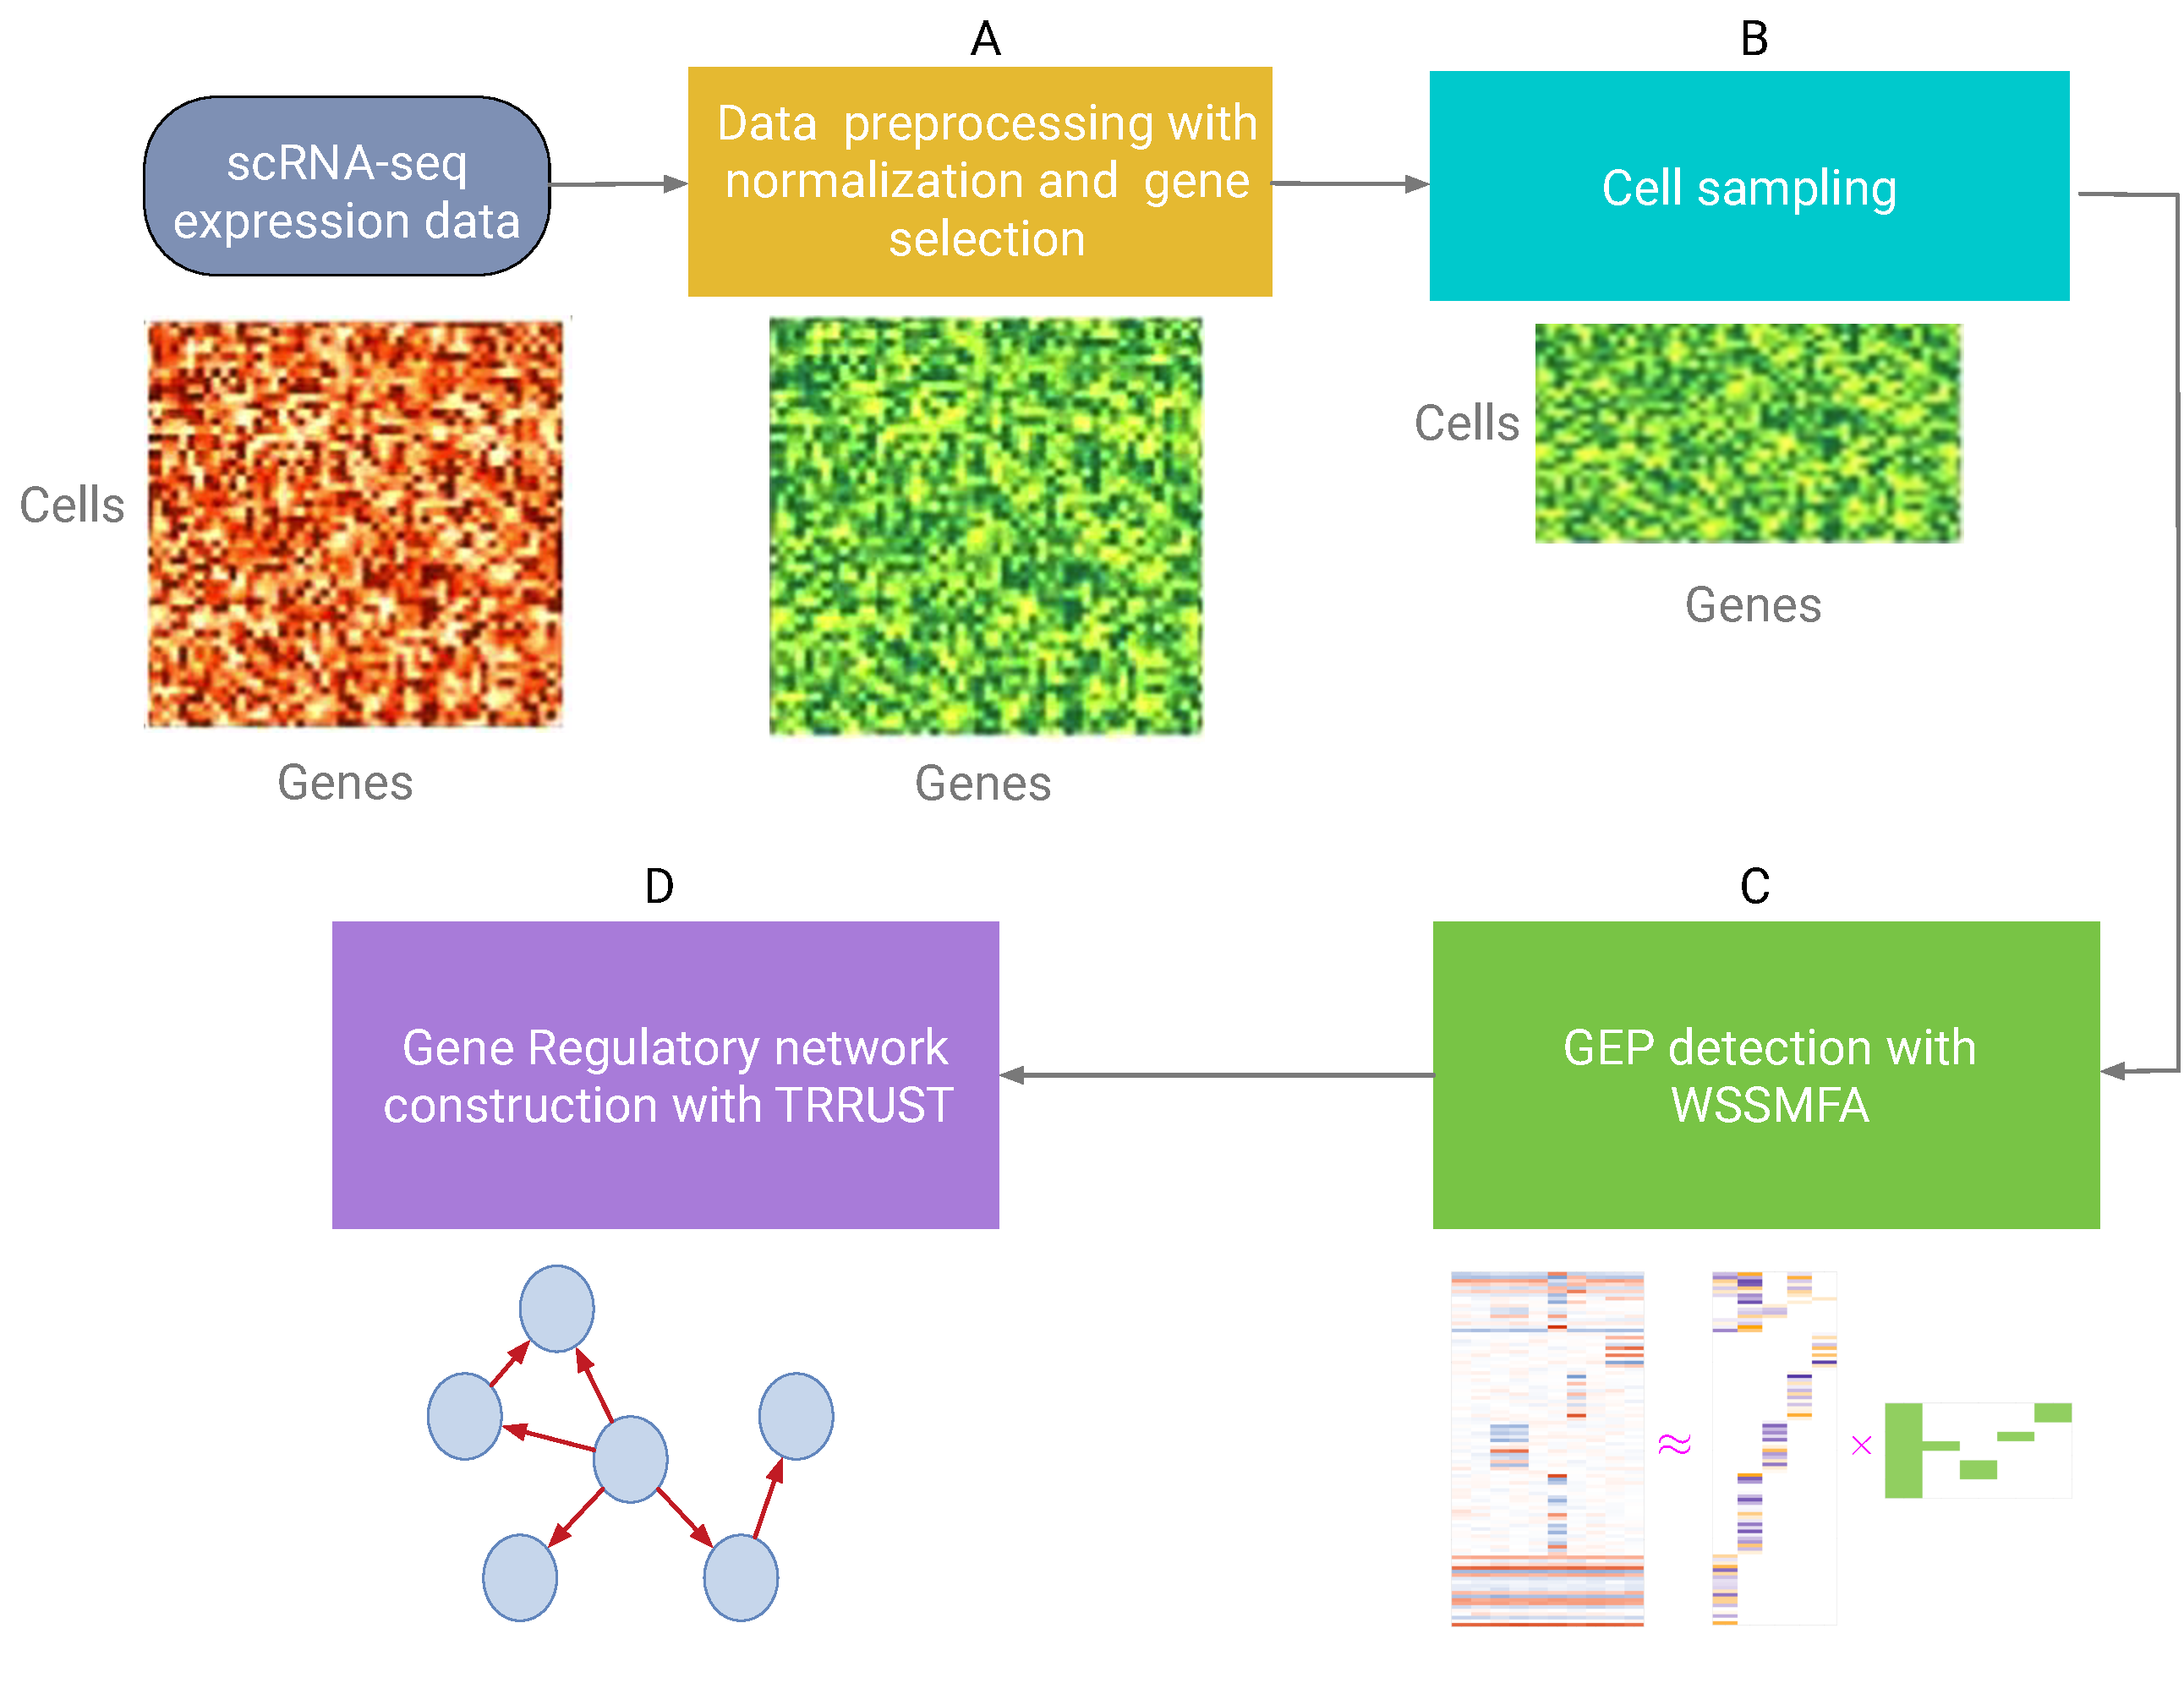
\includegraphics[width=0.4\textwidth]{flowchart-gep.pdf}
    \caption{
        % scGRNHunter flowchart. The input is the scRNA-seq expression data 2D-matrix, whose row stands for cells, column for genes, respectively.
        % (A) Data preprocessing with the input expression data, the output is  a normalized and the column dimension reduced matrix. 
        % Highly expressed genes with a fixed number are chosen for downstream analysis.
        % (B) Cell sampling with a user-defined ratio or a fixed number of cells  from the reduced expression data. 
        % (C) GEP detection with the algorithm WSSMFA. 
        % (D) Gene regulatory network construction with TRRUST.
        scGRNHunter~流程图。输入的是~scRNA-seq~表达数据,用二维矩阵表示,其行代表细胞,列代表基因。
        (A)~用输入的表达数据进行数据预处理,输出的是经过归一化处理且列维度缩小的矩阵。
        选择固定数量的高表达基因进行下游分析。
        (B)~用用户定义的比例或固定数量的细胞从减少的表达数据中进行细胞采样。
        (C)~用~WSSMFA~算法进行~GEP~检测。
        (D)~用~TRRUST~构建基因调控网络。
    }
    \label{fig:gep-flowchart}
\end{figure}
总共包括四个步骤:
\begin{enumerate}
    \item 单细胞数据的预处理,涉及到细胞数据的过滤,归一化,和基因选择;
    \item 单细胞抽样;
    \item GEP~识别,使用我们提出的算法~WSSMFA;
    \item 基因调控网络构建。
\end{enumerate}
下文中我们将详细介绍这四个步骤。

\subsubsection{预处理}
通常假定输入的单细胞数据是二维矩阵, 行代表细胞, 列代表基因, 矩阵中元素值代表细胞中对应基因的表达量。
对于每个数据集, 首先剔除少于~1000~个独特的分子标识符~(UMIs)~检测的细胞,
然后过滤掉平均~500~个细胞中累加没有~1~个~count~的基因。
这个过滤后的计数矩阵我们表示为~$X_{ij}$ ($i~=~1,\ldots, C$~个细胞,$j~=~1,\ldots, G$~个基因)。
然后我们选择由~v-score~\cite{klein2015droplet}~确定的~H~个分散度~(dispersion)~最高的基因作为后续输入。
对于本文中分析的所有数据集上, H~被设置为~500。

在归一化之前选择一个高分散的基因集合是至关重要的, 
因为如果噪声导致的~lower-variance~基因的信号与生物学上有意义的基因信号处在同一个量级上, 那么会对计算不利。 
H~被设置为~500, 主要考虑的是包括足够的基因以检测微妙的生物信号与尽量不包括太多无关基因来加速计算这两方面的权衡。

\subsubsection{细胞抽样}
由于类似于~Drop-seq~等技术使得细胞测序规模比较大, 而且我们在这个方法中主要倾向考虑的对象是基因~(矩阵中的列), 
为了加速计算, 可以约定如果处理的单细胞数据集上细胞的个数大于一个预定的数值, 比如~5000,
我们需要对矩阵的行~(也就是细胞)~采用行随机采样。
如果细胞个数小于预定的数值, 这一步不是必须的, 可以把所有的细胞纳入到后续计算之中。

\subsubsection{加权半非负稀疏矩阵分解算法~WSSMFA}

\begin{figure}[!htbp]
    \centering
    \includegraphics[width=0.9\textwidth]{gep_mf.pdf}
    \caption{
        % Illustration of the algorithm WSSMFA.
        % A.Matrix factorization with the scRNA-seq data 2D-matrix. 
        % B.The objective function, where $W$ is the mask matrix, $\alpha$ and $\lambda$ are sparsity penalty parameters, and C is
        % the number of cells.
        算法~WSSMFA~的说明。
        A. 对~scRNA-seq~数据进行矩阵因子化。
        B.目标函数,其中~W~为掩码矩阵,~$\alpha$~和~$\lambda$~为稀疏度惩罚参数,C~为细胞数。
    }
    \label{fig:gep-mf}
\end{figure}

经过上述步骤处理后的单细胞数据可以表示为一个矩阵~$X_{C \times G}$, $C$~为细胞的数目, $G$~为基因的数目, 
矩阵中的每个值表示该基因在对应的细胞中的表达量。
对于矩阵~$X$, 可以表示为一个因子矩阵~(factor matrix)~$F_{G \times K}$~和一个负荷矩阵~(loading matrix)~$L_{C \times K}$,
并且满足~$X=LF^T$, 如图~\ref{fig:gep-mf} a~所示。 

我们设计了一个具有以下三个特征的矩阵分解目标函数: 
\begin{enumerate}
    \item 对残差加权和的惩罚: 为了考虑基因表达值本身的不确定性,也就是~dropout~效应带来的影响,具有~dropout~值的对应位置处的残差被赋予零权重。
          通过这种方式,基因具有更确定的表达值的对最优参数估计有更大的影响。
    \item 稀疏性: 为了减少过拟合,对分解后的矩阵进行了~$l_1$~惩罚。
    \item 分解矩阵的半非负性: 因子矩阵捕捉组织间的影响模式,因此,使因子矩阵非负易于解释是一个自然约束。
          同时,由于输入矩阵中数值可能有正有负,因此对负荷矩阵没有这样的约束。
\end{enumerate}
基于此,最终的目标函数定义如下~(如图~\ref{fig:gep-mf} b~所示):
\begin{equation}
    \label{eq:obj}
    \min _{F, L} \frac{1}{2 C}\left\|\left(X-L F^{T}\right) \odot W\right\|_{F}^{2}+\alpha\|L\|_{1}+\lambda\|F\|_{1}
\end{equation}
其中,~$F$~是非负的,~$W$~是~binary~掩码矩阵~(mask matrix),~$C$~是细胞个数,
~$\alpha$~和~$\lambda$~是惩罚系数。
$W$~跟~$X$~的维度相同,并且有:
\begin{equation}
    W_{i j}=\left\{\begin{array}{ll}1 & \text { if } x_{i j}>0 \\ 0 & \text { otherwise }\end{array}\right.
\end{equation}

这个目标函数是双凸~(biconvex)~的, 也就是说, 只在~$F$~中凸, 或者只在给定的~$L$~中凸, 但在两者共同存在时不凸。
我们使用交替最小二乘法~(ALS, alternating least squares)~与梯度下降~(gradient descent)~法来优化目标函数~(算法~\ref{alg:wssmfa}, 在~R~版本~3.5.1~中实现~\cite{goeman2012penalized,goeman2010l1})。
在每一次迭代中我们固定~F~并更新~L, 然后固定~L~并更新~F, 当两次迭代之间~F~的差值的~Frobenius~范数~<~0.01~时, 更新结束。
在每一步更新中, 优化问题都是有约束条件的线性回归。
由于线性回归的解保证了均方误差与惩罚之和最小, 所以代价函数单调下降。
\begin{algorithm}
    \caption{Weighted semi-nonnegative sparse matrix factorization algorithm~(WSSMFA)}
    \label{alg:wssmfa}
    \begin{algorithmic}[1]
        \State Input: $X_{G \times C}$                                   \Comment{$G$ genes, $C$ cells}
        \State Output: $L_{G \times K}$, $F_{C \times K}$                \Comment{Loading matrix and factor matrix}
        \While{not converged}
            \For{$i = 1 \to G$}                                           
                \State $l_{i} \leftarrow \min _{l_{i}}\left\|\left(x_{i}-l_{i} F^{T}\right) \odot w_{i}\right\|_{F}^{2}+\alpha\left\|l_{i}\right\|_{1}$
                \State which is equivalent to 
                \State $l_{i} \leftarrow \min _{l_{i}}\left\|x_{i} \odot w_{i}-l_{i}\left(F^{T} \operatorname{diag}\left(w_{i}\right)\right)\right\|_{F}^{2}+\alpha\left\|l_{i}\right\|_{1}$
            \EndFor
            \For{$j = 1 \to C$}
                \State $f_{j} \leftarrow \min _{f_{j}}\left\|\left(x_{j}-f_{j} L^{T}\right) \odot w_{j}\right\|_{F}^{2}+\lambda \mid f_{j}\left\|_{1},\right\| f_{j} \| \geq 0$
                \State which is equivalent to 
                \State $f_{j} \leftarrow \min _{f_{j}}\left\|\left(x_{j} \odot w_{j}-f_{j}\left(L^{T} \operatorname{diag}\left(w_{j}\right)\right)\right)\right\|_{F}^{2}+\lambda\left\|f_{j}\right\|_{1},\left\|f_{j}\right\| \geq 0$
            \EndFor
        \EndWhile           
  \end{algorithmic}
\end{algorithm}

\subsubsection{构建基因调控网络}
TRRUST~(version 2,~\cite{han2018trrust})~是一个采用数据挖掘辅助建立的人类和小鼠转录调控网络数据库,并提供了网页版本的服务。
当前版本的~TRRUST~分别包含~800~个人类~TFs~(调控因子)~和~828~个小鼠~TFs~的~8,444~和~6,552~个~TF-target~调控关系。
TRRUST~数据库还提供了调控模式的信息~(激活或抑制)。
目前已知调控模式的调控关系有~8972~个~(59.8\%)。

针对因子矩阵~(factor matrix)~$F_{G \times K}$, 每一个因子代表了一个~GEP, 
身份~GEPs~里面的基因没有交集, 活动~GEPs~跟各个身份~GEP~之间一般存在相交的基因, 
针对身份~GEP~和活动~GEP~我们根据基因列表可以在~TRRUST~线上服务上查询关键的调控因子,然后构建基因调控网络。
%根据~GEP~结合~TRRUST~数据库找到~TF, 然后构建得到整个的基因调控网络。

\subsection{实验数据}
本文中使用的数据集如表~\ref{tab:dataset}所示。
\begin{table}[!htbp]
    \caption{\label{tab:dataset}使用的公开数据集} 
    \resizebox{\columnwidth}{!}{%  
    \begin{tabular}{lllll}
    \hline
    Author(s)                           & Year & Dataset title                                                                                                              & Dataset URL                                                                                               & Database and Identifier                                                                          \\ \hline
    \multicolumn{1}{c}{Quadrato G, et.} & 2017 & \begin{tabular}[c]{@{}l@{}}Cell diversity and network \\ dynamics in photosensitive \\ human brain organoids.\end{tabular} & \begin{tabular}[c]{@{}l@{}}https://www.ncbi.nlm.nih.gov\\ /geo/query/acc.cgi?\\ acc=GSE86153\end{tabular} & \multicolumn{1}{c}{\begin{tabular}[c]{@{}c@{}}Gene Expression Omnibus, \\ GSE86153\end{tabular}} \\
    \end{tabular}
    }
\end{table}

\subsection{实验结果}
\subsubsection{模型选择}
我们需要设置~WSSMFA~算法的超参数,包括因子个数~($K$)~和稀疏惩罚参数~($\alpha$,$\lambda$)。
我们在~[20,25,30,35,40]~范围内评估~$K$, 在~[4.9,24.5,49,245,490]~范围内评估~$\alpha$~和~$\lambda$。
这些范围的选择是通过考虑单细胞中的一些已知的先验知识比如类别数来定义~$K$~的可信值,
并通过手动检查~$\alpha$~和~$\lambda$~变化很大的范围,
以避免对这些超参数的范围进行高分辨率搜索,导致明显不合理的解,
如因子缺乏稀疏性或者大量为空,或者与原始数据间没有关联性。

在指定的搜索空间内,我们利用~(1)~之前定义的矩阵分解稳定性标准和~(2)~学习因子的独立性,即代表足够的稀疏性,
对所有~$K$、$\alpha$~和~$\lambda$~组合的模型进行了评估。
考虑到矩阵因子化的随机性, Brunet~等人提出了一种寻找最稳定的因子化结果的方法,
这种方法已经在各种研究中得到应用~\cite{brunet2004metagenes,wu2016stability}。
我们对每个模型进行随机初始化,运行~30~次后得到共识矩阵~$C$。
$C$~中的值在~$0$~和~$1$~之间,代表一对细胞被分配到同一个因子的比例。
利用~$C$~矩阵, 我们计算了共识相关性, 用于衡量~$C$~矩阵的离散程度。
共识相关度越高, 说明因子矩阵越稳定。

在这里,对于每一个观察到的学习到的非空因子~$K^\textup{'}$~的平均数~(可能小于输入的~$K$~),
我们对~$\lambda$~和~$\alpha$~的不同取值进行了汇总,
并计算了中位共线性相关性~(cophenetic correlation,\cite{brunet2004metagenes})。
我们从考虑中剔除了任何对应于~K~的中位共时相关性~$< 0.9$~的~$K^\textup{'}$。
接下来,在剩下的单个设置中,我们排除任何一个共线性相关性~$< 0.9$~的参数取值。
最后,在这些明显稳定的设置中,我们根据因子对之间的最小皮尔逊相关性选择最终的超参数,
使得独立的因子和与数据中独立信号的稀疏程度相匹配。
在这里,我们计算了每对因子的皮尔逊相关性, 取了对偶相关矩阵的~Frobenius norm, 
并在~30~个相同设置的随机初始化运行中取平均值。

\subsubsection{WSSMFA~揭示了~GEPs~的存在}
在大脑类器官数据集上,我们在数据预处理之后保留了~500~个分散度最高的基因~($H = 500$),
按照~0.05\%~的比例随机抽取了~2623~个细胞,按照模型选择的准则操作后,
最终确定~$K = 15$,~$\alpha = 50$,~$\lambda = 5$, 
即~15~个因子~(f1,~f2, $\ldots$,~f15), 也就是对应~15~个~GEP。
负荷矩阵~$L$~揭示了各细胞的表达量与因子之间的组合线性关系, 我们按照细胞类别对负荷矩阵进行统计,
针对每个~GEP~我们可以画出对应类别的负荷的箱形图~(boxplot), 如图~\ref{fig:gep-gep}所示。
另外,为了辅助说明, 我们也对该单细胞数据结合已知的细胞的标注类别信息使用基于~t~分布的随机邻域嵌入~(t-SNE)~进行二维可视化,
t-SNE~图反应了单细胞数据中细胞分布的宏观结构,可以看出单细胞数据是否有不同的类别,即细胞是否存在异质性。
结合该数据集提供的细胞类别标签,我们对抽样之后的数据可视化,如图~\ref{fig:gep-tsne}所示。

\begin{figure}[!htbp]
    \centering
    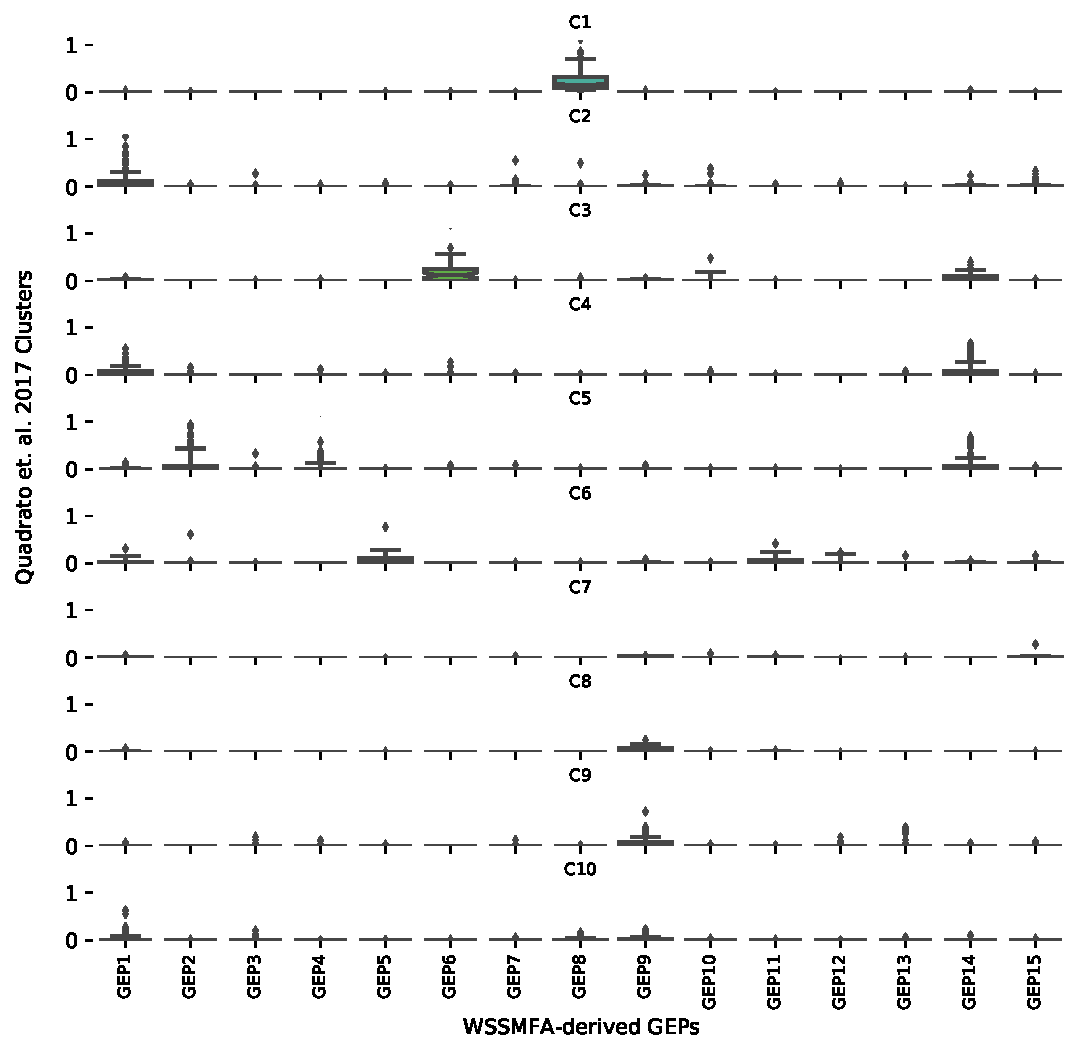
\includegraphics[width=0.9\textwidth]{GEP_Usage_Vs_Published_Clusters_QuadratoEtAI.pdf}
    \caption{
    % GEPs detected with WSSMFA.
    % GEP1,~GEP2, $\ldots$,~GEP15 are the 15 GEPs derived with WSSMFA algorithm.
    % For each GEP, the loading values based on the 10 different clusters,i.e. C1, C2, $\ldots$, C10,  are visualized with boxplot.
    用~WSSMFA~检测的~GEPs。
    GEP1,~GEP2,$\ldots$,~GEP15~是用~WSSMFA~算法得出的~15~个~GEP。
    对于每个~GEP,根据~10~个不同的聚类,
    即~C1,~C2,$\ldots$,~C10,用箱形图直观地显示出其负载值。 
    }
    \label{fig:gep-gep}
\end{figure}


\begin{figure}[!htbp]
    \centering
    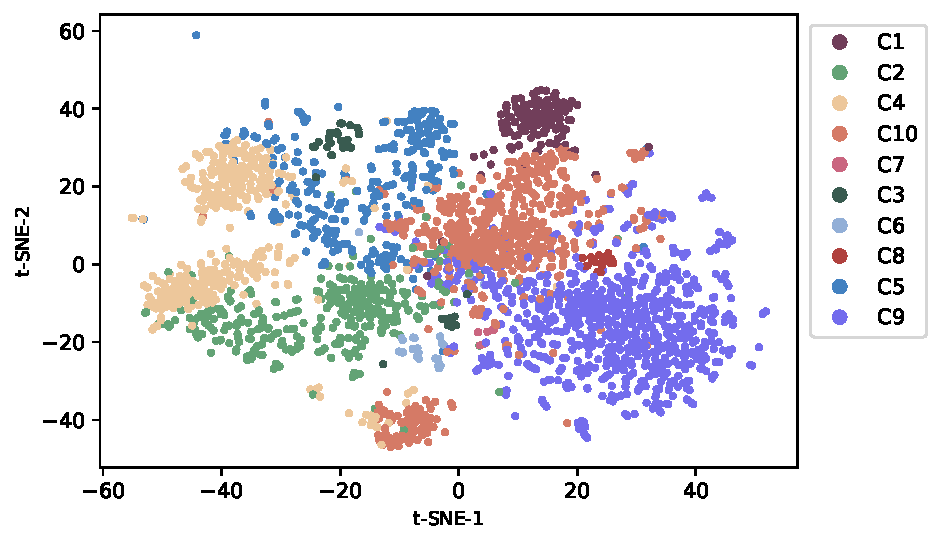
\includegraphics[width=0.9\textwidth]{tsne_Clusters_QuadratoEtAI.pdf}
    \caption{
    %The sampled brain organisms data visualized with t-SNE.
    采样后的大脑器官数据使用~t-SNE~可视化
    }
    \label{fig:gep-tsne}
\end{figure}

如果一个~GEP~仅仅在一个细胞类别中表达,很显然它就是一个身份~GEP;
如果在两个或者多个细胞类别中表达,那么它就属于活动~GEP。
结合图~\ref{fig:gep-gep}~和图~\ref{fig:gep-tsne}~可以看出, 
GEP6~和~GEP8~是典型的身份~GEPs~(分别对应到类别~C3~和~C1), GEP1、GEP9~和~GEP14~是典型的活动~GEPs。
GEP1~牵涉到类别~C2,~C4,~C6~和~C10; GEP14~牵涉到类别~C3,~C4,~C5。

\subsubsection{身份调控网络与活动调控网络的构建}
结合因子矩阵~$F$,每一列中系数不为零的基因即是该因子~(也就是~GEP)~中所包含的基因,
针对每个~GEP,我们可以结合~TRRUST~(version 2)~构建其调控网络。
如图所示,即为每个~GEP~所对应的大脑类器官数据集上的基因调控网络。

由~GEP6~构建的基因调控网络如图~\ref{fig:gep-grn-gep6}~所示:
\begin{figure}[!htbp]
    \centering
    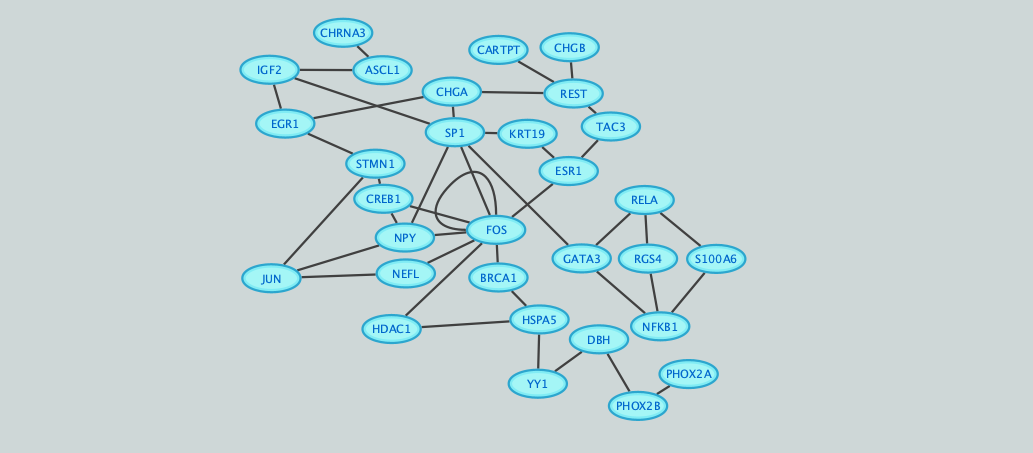
\includegraphics[width=0.95\textwidth]{GEP6.key_regulators.tsv.cs.network.tsv.png}
    \caption{
    %The gene regulatory network of GEP6, constructed with the TRRUST database.
    结合~TRRUST~数据库构建的~GEP6~的基因调控网络
    }
    \label{fig:gep-grn-gep6}
\end{figure}

由~GEP8~构建的基因调控网络如图~\ref{fig:gep-grn-gep8}~所示:
\begin{figure}[!htbp]
    \centering
    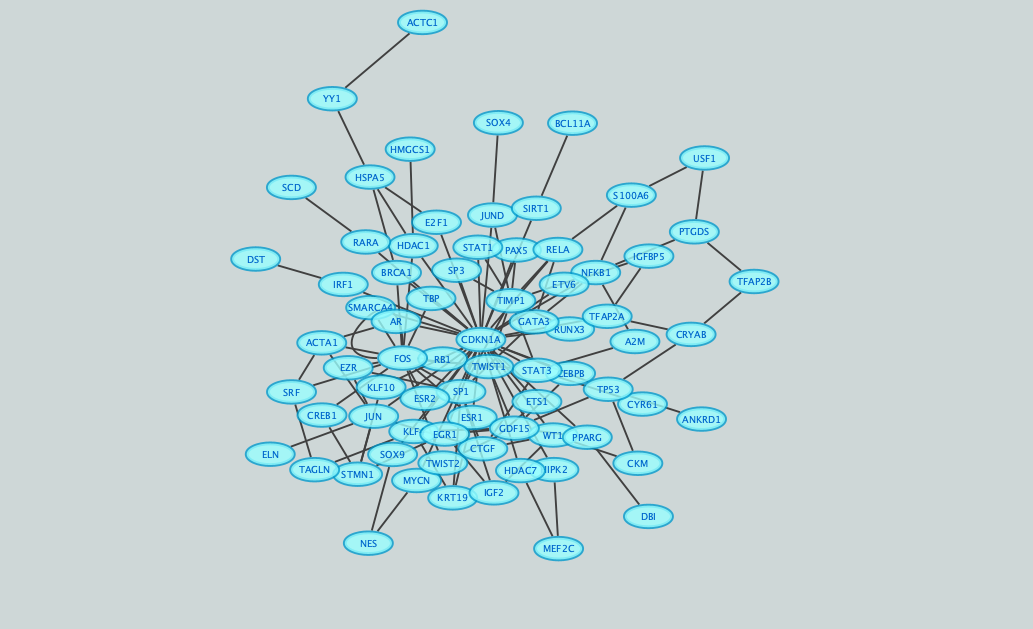
\includegraphics[width=0.95\textwidth]{GEP8.key_regulators.tsv.cs.network.tsv.png}
    \caption{
    %The gene regulatory network of GEP8, constructed with the TRRUST database.
    结合~TRRUST~数据库构建的~GEP8~的基因调控网络
    }
    \label{fig:gep-grn-gep8}
\end{figure}

由~GEP14~构建的基因调控网络如图~\ref{fig:gep-grn-gep14}~所示:
\begin{figure}[!htbp]
    \centering
    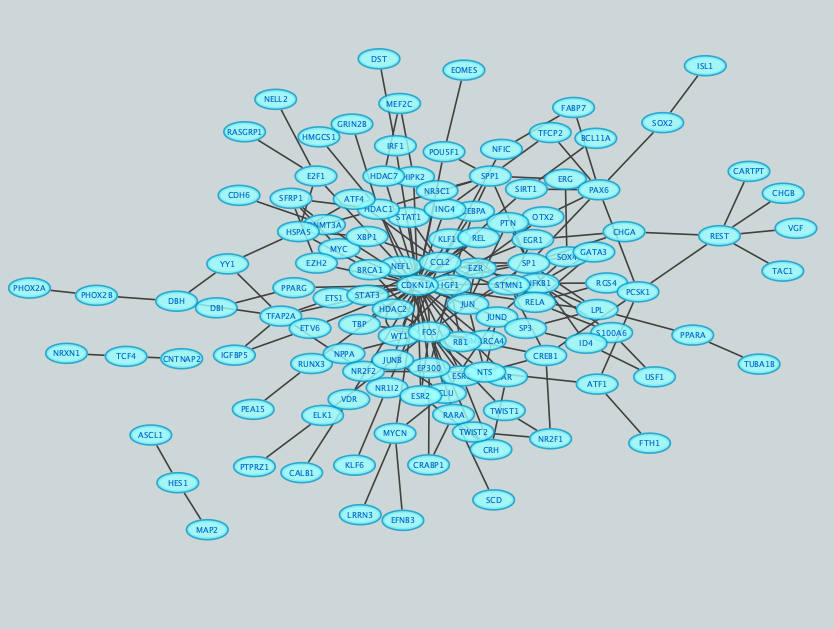
\includegraphics[width=0.95\textwidth]{GEP14.key_regulators.tsv.cs.network.tsv.png}
    \caption{
    %The gene regulatory network of GEP14, constructed with the TRRUST database.
    结合~TRRUST~数据库构建的~GEP14~的基因调控网络
    }
    \label{fig:gep-grn-gep14}
\end{figure}

\subsection{讨论}
scGRNHunter的核心算法依赖~WSSMFA~这个矩阵分解方法, 该方法的一个基本限制是前提假设, 
即细胞的表达可以被建模为~GEPs~的线性组合。
值得注意的是, 这排除了转录抑制的建模, 也就是说其中一个或多个基因将被一个~GEP~诱导,
当第二个抑制~GEP~在同一细胞中活跃时, 其表达量会显著降低。
据我们所知, 这种关系还没有在矩阵因子化框架中表示, 但它们可能更容易纳入新的潜变量模型类别,
如变分自动编码器~(VAEs)~\cite{ding2018interpretable,gronbech2018scvae}。
VAEs~代表了一个高度灵活的隐式空间中的单元, 可以捕捉隐式变量之间的非线性和相互作用。
然而, 虽然隐变量的设计是为了促进输入基因表达数据的准确重建, 
但它们是否可以直接或间接地解释为不同的~GEPs~相互作用, 还有待证明。
在可预见的未来, 需要综合权衡考虑模型本身的灵活性与训练和解释它们的输出的难度这两个方面。

随着~RNA~捕获效率和通量的不断技术进步, scRNA-Seq~数据可能会变得更加丰富和广阔。
这将使得检测越来越细微的~GEPs~成为可能, 从而捕捉细胞类型、细胞状态和活动的生物变异性。
在这里, 我们已经展示了一个计算方法框架~scGRNHunter, 
可以用来直接从~scRNA-Seq~中推断出这样的~GEPs, 
而不需要进行实验操作, 从而为细胞和组织行为提供了至关重要的解释, 
并为基因调控网络的构建提供了一个全新的思路。